% $Header$

\documentclass{beamer}

\mode<presentation>
{
  \usetheme{default}
  \setbeamercovered{transparent}
}


\usepackage[english]{babel}

\usepackage[latin1]{inputenc}

\usepackage{times}
\usepackage[T1]{fontenc}
\usepackage{subfig}
\usepackage{amssymb}
\usepackage{amsmath}
\usepackage{mathtools}

\graphicspath{{../figures/}}

\newcommand*{\transpose}{^{\mkern-1.5mu\mathsf{T}}}

\title
{Evaluation of an Appearance-Preserving Mesh Simplification Scheme}

\author
{Rasmus Hedin}

\institute[Link�pings Universitet]
{
  Department of Electrical Engineering\\
  Link�pings Universitet
}

\date
{2018-06-15}


% If you have a file called "university-logo-filename.xxx", where xxx
% is a graphic format that can be processed by latex or pdflatex,
% resp., then you can add a logo as follows:

\pgfdeclareimage[height=0.5cm]{university-logo}{../figures/liu_primary_black_sv.pdf}
\logo{\pgfuseimage{university-logo}}



% Delete this, if you do not want the table of contents to pop up at
% the beginning of each subsection:
\AtBeginSubsection[]
{
  \begin{frame}<beamer>{Outline}
    \tableofcontents[currentsection,currentsubsection]
  \end{frame}
}


% If you wish to uncover everything in a step-wise fashion, uncomment
% the following command: 

% \beamerdefaultoverlayspecification{<+->}


\begin{document}
\captionsetup[subfloat]{labelformat=empty}

\begin{frame}
  \titlepage
\end{frame}

\begin{frame}{Outline}
  \tableofcontents
  % You might wish to add the option [pausesections]
\end{frame}


% Since this a solution template for a generic talk, very little can
% be said about how it should be structured. However, the talk length
% of between 15min and 45min and the theme suggest that you stick to
% the following rules:  

% - Exactly two or three sections (other than the summary).
% - At *most* three subsections per section.
% - Talk about 30s to 2min per frame. So there should be between about
% 15 and 30 frames, all told.

\section{Introduction}

\subsection[Short First Subsection Name]{First Subsection Name}

\begin{frame}{Make Titles Informative. Use Uppercase Letters.}{Subtitles are optional.}
  \begin{itemize}
  \item Item 1

  \item Item 2

  \end{itemize}
\end{frame}


\subsection{Second Subsection}

\begin{frame}{Make Titles Informative.}
\end{frame}

\begin{frame}{Make Titles Informative.}
\end{frame}

\section{Implementation}
% == Figures ==
% mesh transformations
% plane point distance
% qem
% quadric planes
\begin{frame}{Quadric Error Metric}
  \begin{itemize}
  \item Iteratively perform edge collapses
  \item Cost based on distance to neighboring faces' planes
  \end{itemize}
  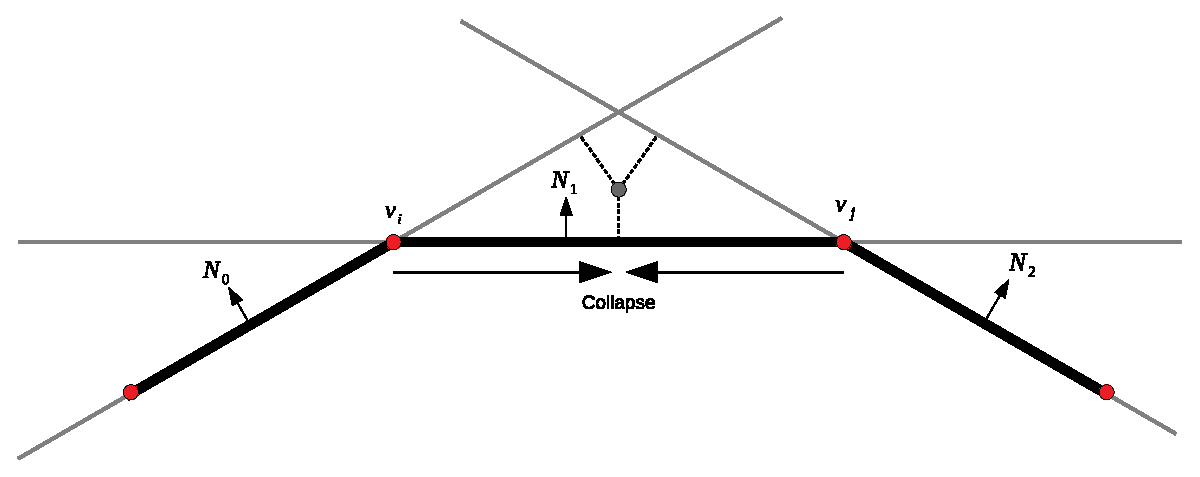
\includegraphics[width=\linewidth]{qem_precontract.eps}
\end{frame}

\begin{frame}{Quadric Error Metric}
  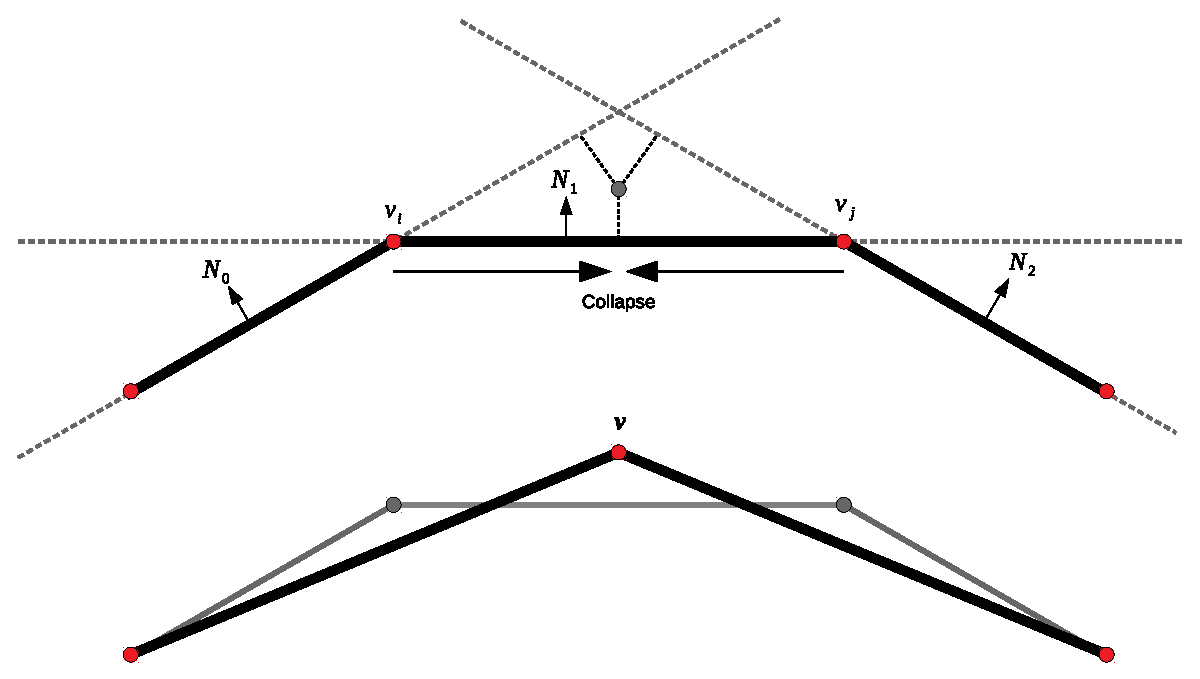
\includegraphics[width=\linewidth]{qem.eps}
\end{frame}

\begin{frame}{Quadric Error Metric}
  Squared distance from point \(v\) to plane \(f\)
  \begin{equation*}
    \mathbf{v} = [x, y, z, 1]\transpose,~\mathbf{f} = [a, b, c, d]\transpose
  \end{equation*}
  \begin{align*}
    D^2 &= (\mathbf{f}\transpose\mathbf{v})^2\\
    &= \mathbf{v}\transpose(\mathbf{f}\mathbf{f}\transpose)\mathbf{v}\\
    &= \mathbf{v}\transpose\mathbf{Q}\mathbf{v}
  \end{align*}
  \begin{equation*}
    Q_f =
    \begin{bmatrix}
      a^2 & ab  & ac  & ad \\
      ab  & b^2 & bc  & bd \\
      ac  & bc  & c^2 & cd \\
      ad  & bd  & cd  & d^2
    \end{bmatrix}
  \end{equation*}
\end{frame}

\begin{frame}
  Sum of distances to planes \(f_k\) of triangles in \(v_i\)'s neighborhood
  \begin{columns}
    \begin{column}{.52\linewidth}

      \begin{align*}
        D^2 &= \sum_k{\mathbf{v}_i\transpose\mathbf{Q}_k\mathbf{v}_i}\\
            &= \mathbf{v}_i\transpose\left(\sum_k{\mathbf{Q}_k}\right)\mathbf{v}_i\\
            &= \mathbf{v}_i\transpose\mathbf{Q}_i\mathbf{v}_i
      \end{align*}
    \end{column}
    \begin{column}{.48\linewidth}
      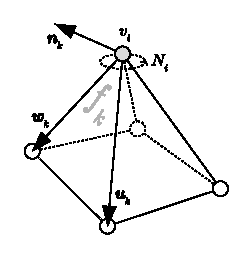
\includegraphics{quadric_planes.eps}
    \end{column}
  \end{columns}
\end{frame}

\begin{frame}
  Finding optimal position for \(v_i\)
  \begin{equation*}
    \begin{bmatrix}
      q_{11} & q_{12}  & q_{13}  & q_{14} \\
      q_{21} & q_{22}  & q_{23}  & q_{24} \\
      q_{31} & q_{32}  & q_{33}  & q_{34} \\
      0      & 0       & 0       & 1
    \end{bmatrix}
    \bar{\mathbf{v}}_i
    =
    \begin{bmatrix}
      0\\
      0\\
      0\\
      1     
    \end{bmatrix}
      \end{equation*}
\end{frame}

\begin{frame}{Quadric Error Metric}
  Initialization
  \begin{enumerate}
  \item Compute \(4x4\) matrix \(Q\) for each vertex
  \item Compute optimal vertex position for each edge collapse
  \item Compute cost of each edge collapse
  \item Store edge collapses in min-heap with cost as key
  \end{enumerate}

  Simplification
  \begin{enumerate}
  \item Collapse edge on top of min-heap
  \item Recompute optimal positions and costs
  \item Repeat  
  \end{enumerate}
\end{frame}


\begin{frame}{Quadric Error Metric}

  \begin{columns}
    \begin{column}{.52\linewidth}
      
      \begin{equation}
        \mathbf{f}_k: \mathbf{n}_k\transpose\mathbf{v}_i + d = 0
      \end{equation}
      \begin{equation}
        \mathbf{Q}_i = \sum_{f_k \in N_i}  \mathbf{f_k} \mathbf{f_k}\transpose
      \end{equation}
      \begin{equation}
        \Delta(\mathbf{v}) = \mathbf{v}\transpose\mathbf{Q}\mathbf{v}
      \end{equation}
    \end{column}%
    \begin{column}{.48\linewidth}
      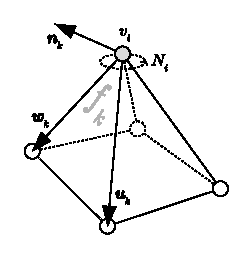
\includegraphics{quadric_planes.eps}
    \end{column}
  \end{columns}
\end{frame}

\begin{frame}{Quadric Error Metric}
  \begin{columns}
    \begin{column}{.52\linewidth}
      \begin{align}
        \begin{split}
          D^2 &= (\mathbf{n}\transpose\mathbf{v} + d)^2\\
          &= \mathbf{v}\transpose(\mathbf{nn}\transpose)\mathbf{v} + 2d\mathbf{n}\transpose\mathbf{v} + d^2
        \end{split}
      \end{align}
      \begin{align}
        \begin{split}
          Q &= (\mathbf{nn}\transpose, d\mathbf{n}, d^2)\\
          &= (\mathbf{A}, \mathbf{b}, c)
        \end{split}
      \end{align}

      \begin{equation}
        \mathbf{A}\mathbf{v} + \mathbf{b} = 0
      \end{equation}
      \begin{equation}
        Q(\mathbf{v}) = \mathbf{v}\transpose\mathbf{A}\mathbf{v} + 2\mathbf{b}\transpose\mathbf{v} + c
      \end{equation}
    \end{column}%
    \begin{column}{.48\linewidth}
      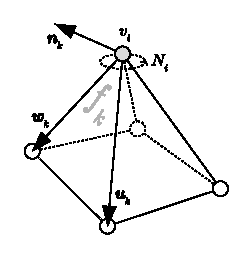
\includegraphics{quadric_planes.eps}
    \end{column}
  \end{columns}
\end{frame}

% wedge vertex
% pyramid
% pull filter
% push filter



\section{Evaluation}
% == Figures ==
% rhombicuboctahedron
% volume


\section{Results}
% luminance
\begin{frame}{Rms Luminance Error}
  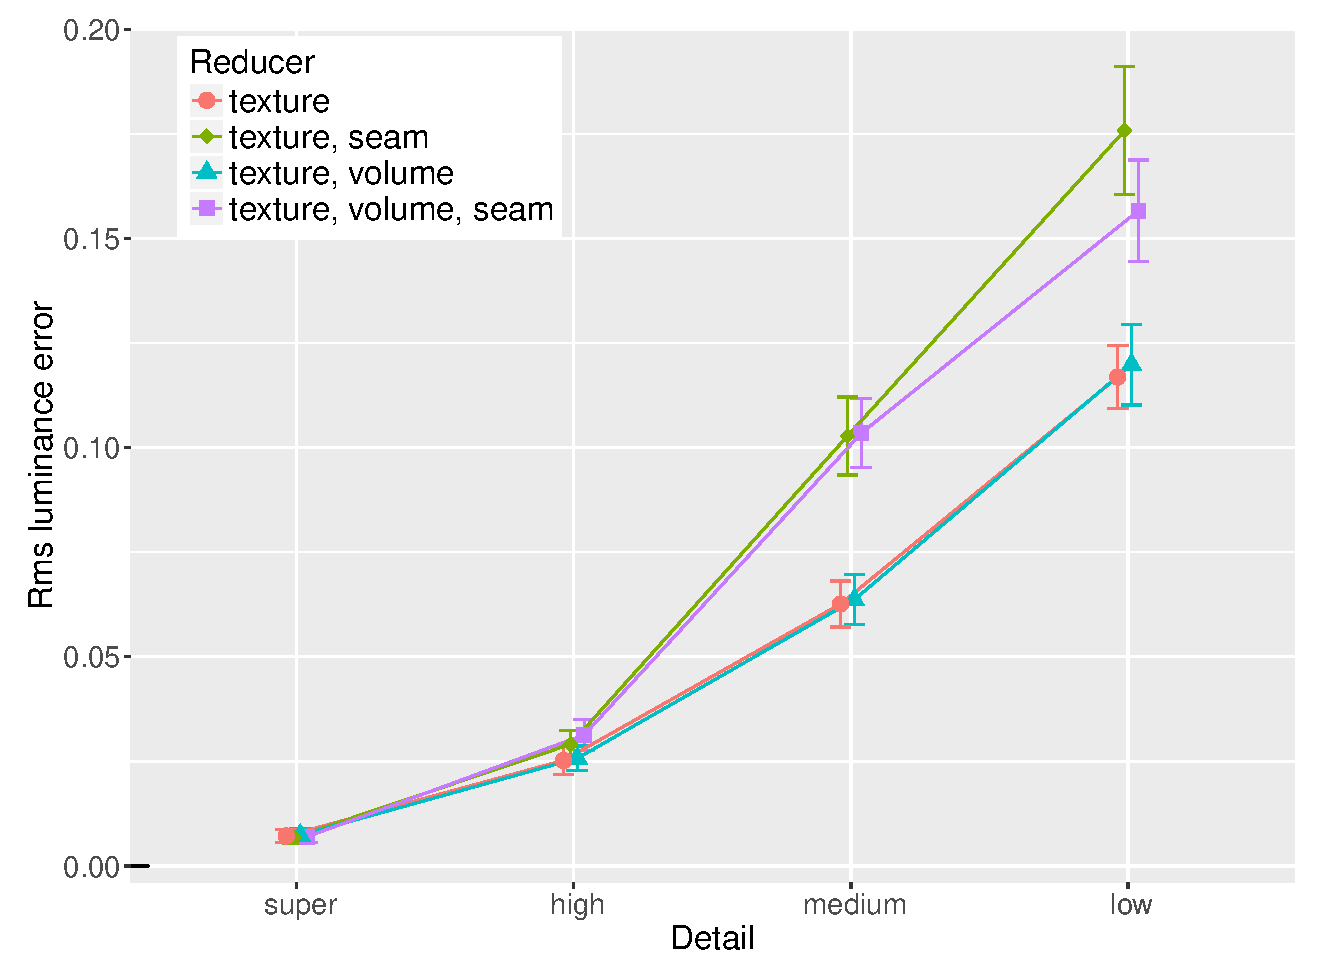
\includegraphics[width=.9\linewidth]{Rdata/rms_luminance.eps}
\end{frame}

% color and geometry
\begin{frame}{Geometric Error}
  \begin{figure}
    \subfloat[Rms geometric error]{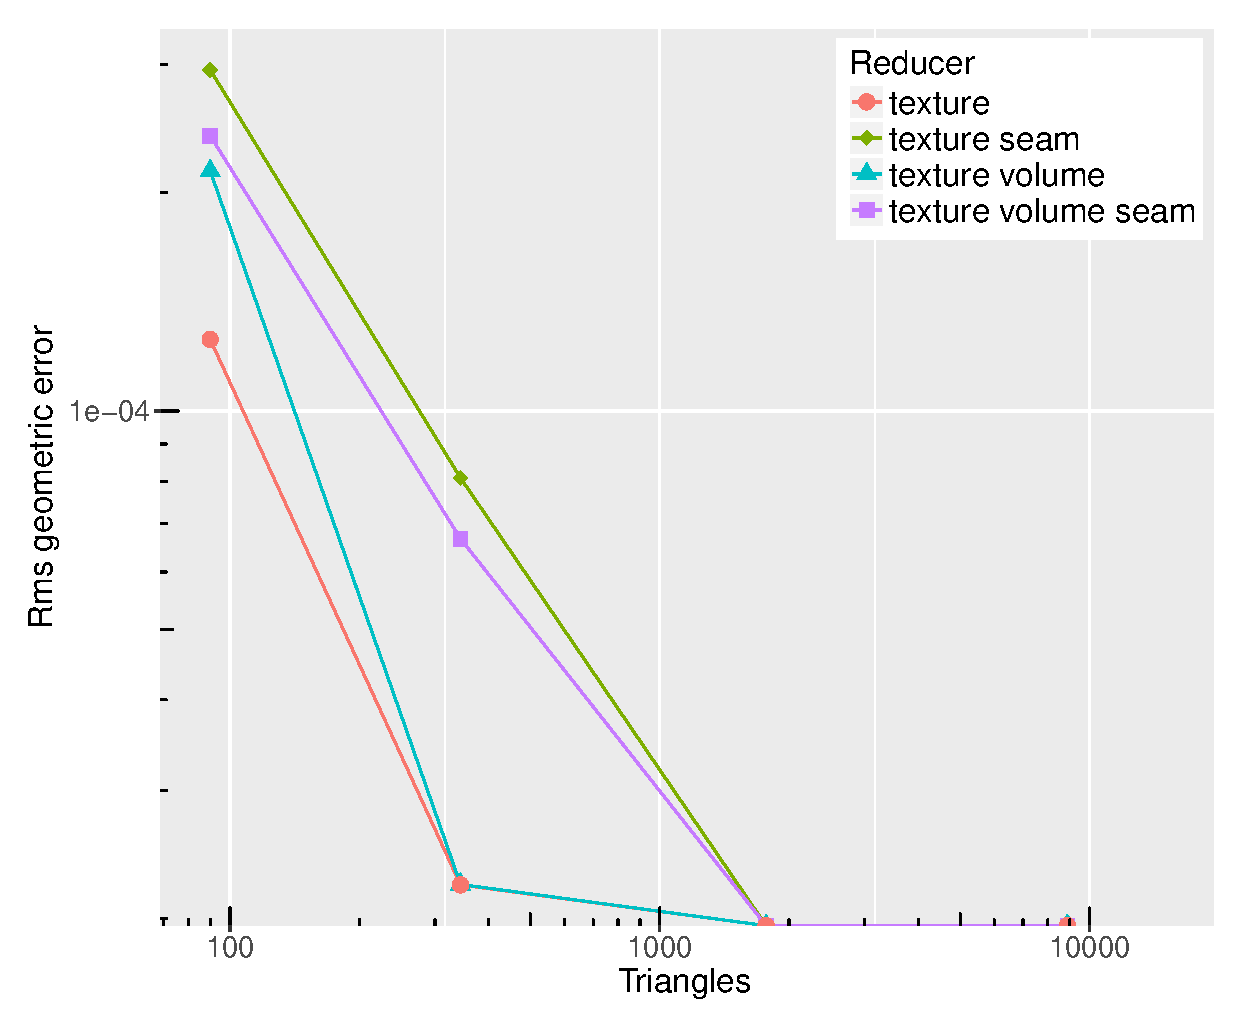
\includegraphics[width=.5\linewidth]{Rdata/rms_geometric_800.eps}}
    \subfloat[Max geometric error]{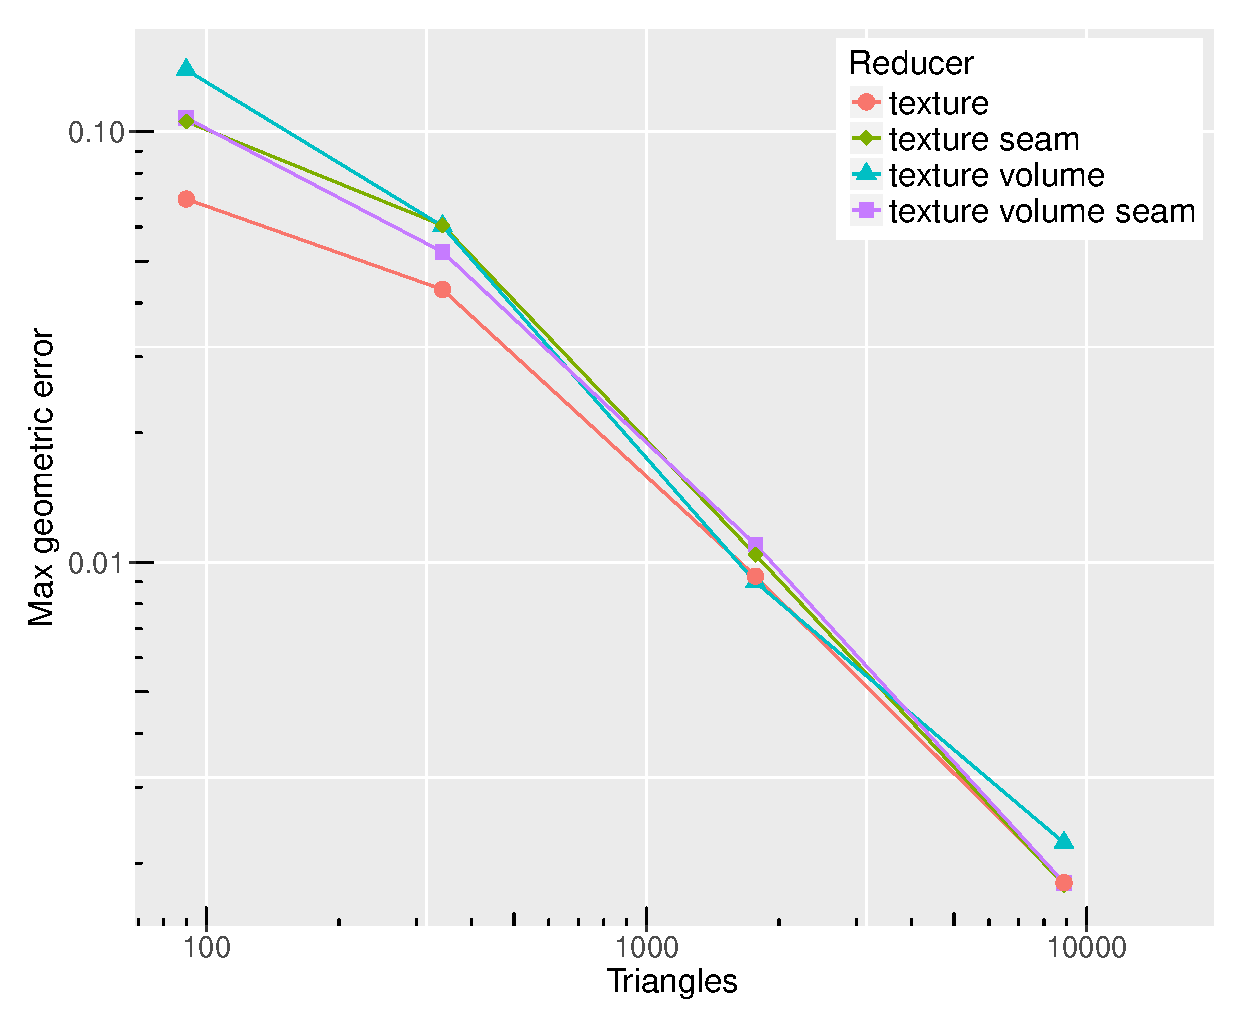
\includegraphics[width=.5\linewidth]{Rdata/max_geometric_800.eps}}
  \end{figure}
\end{frame}

\begin{frame}{Color error}
  \begin{figure}
    \subfloat[Rms color error]{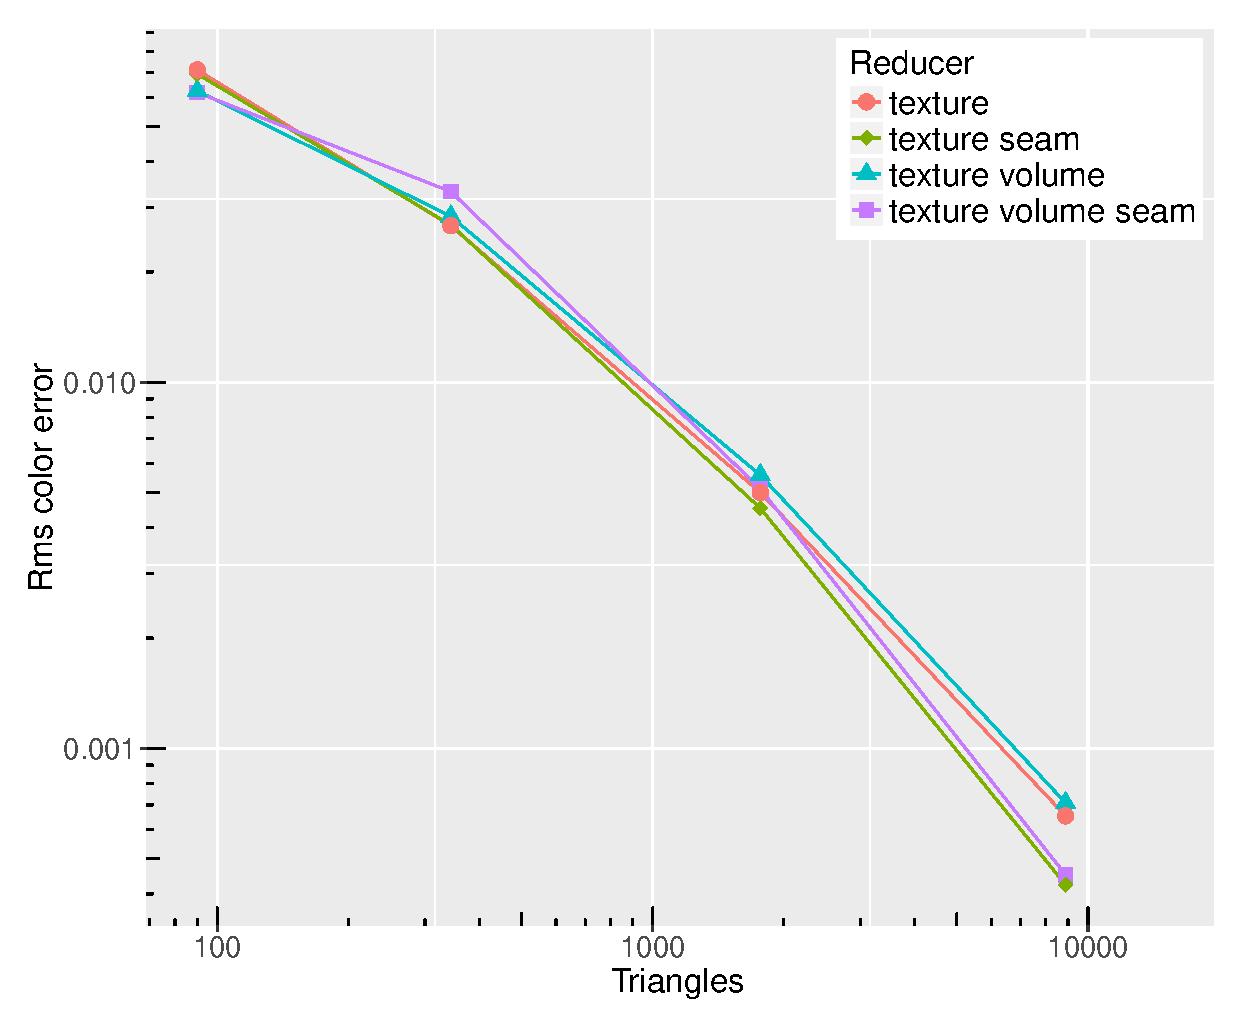
\includegraphics[width=.45\linewidth]{Rdata/rms_color_800.eps}}
    \subfloat[Max color error]{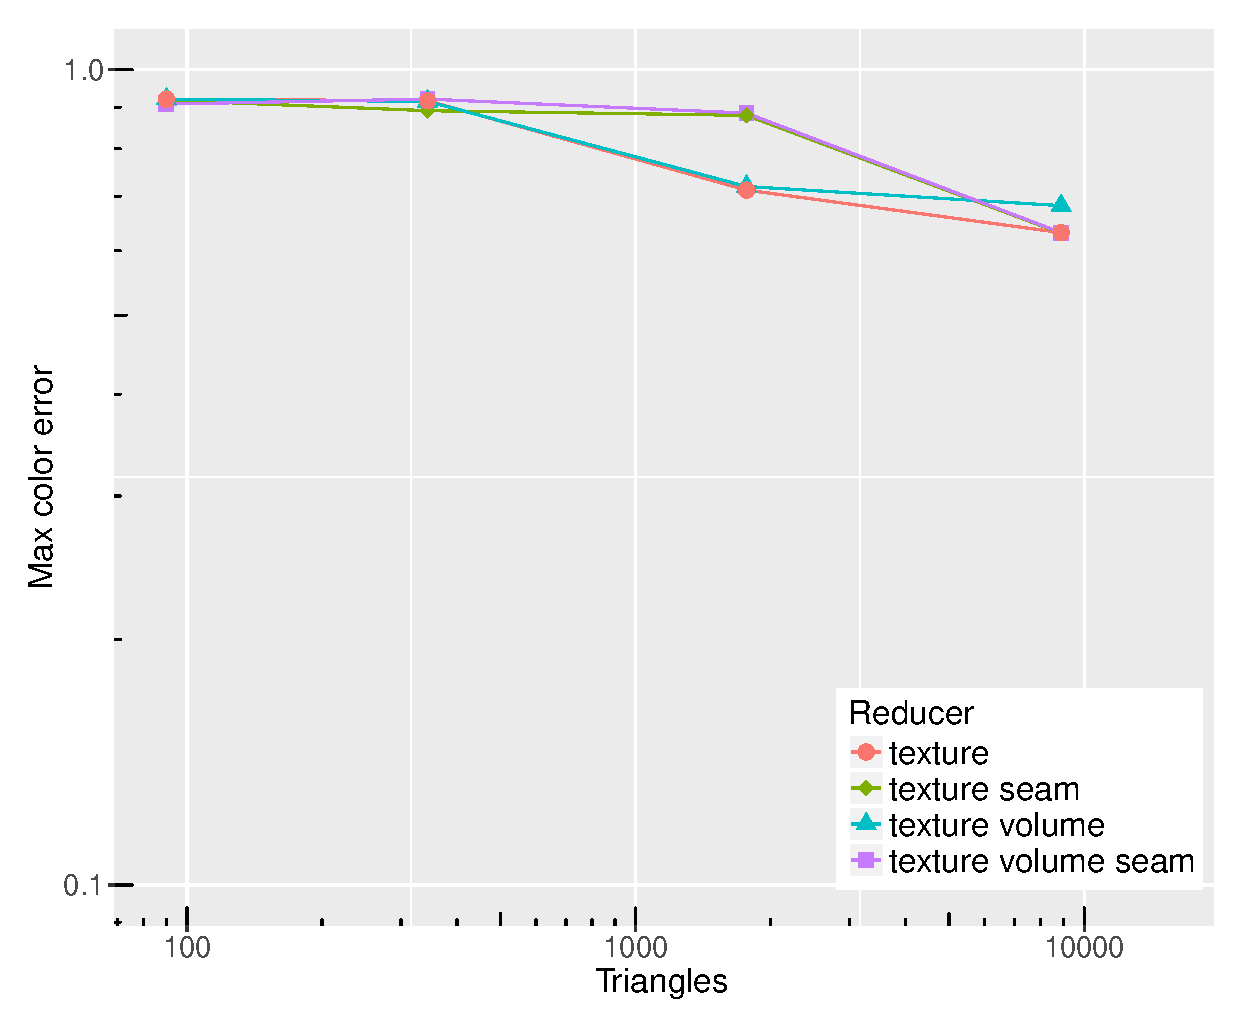
\includegraphics[width=.45\linewidth]{Rdata/max_color_800.eps}}
  \end{figure}
\end{frame}

% volume
\begin{frame}{Volume}
  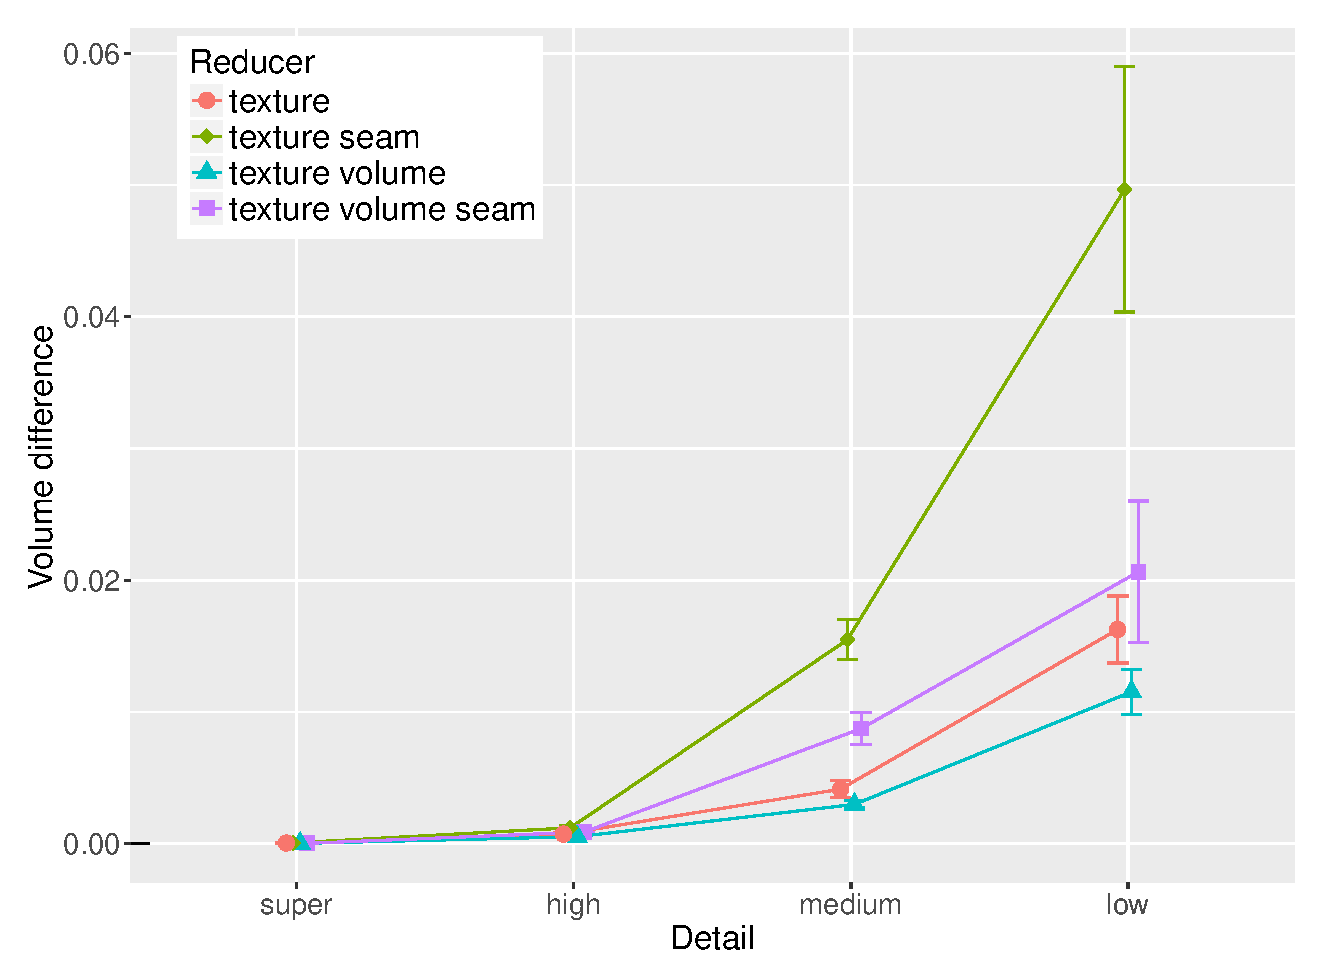
\includegraphics[width=.9\linewidth]{Rdata/volume_diff.eps}
\end{frame}

\begin{frame}{Execution Time}
  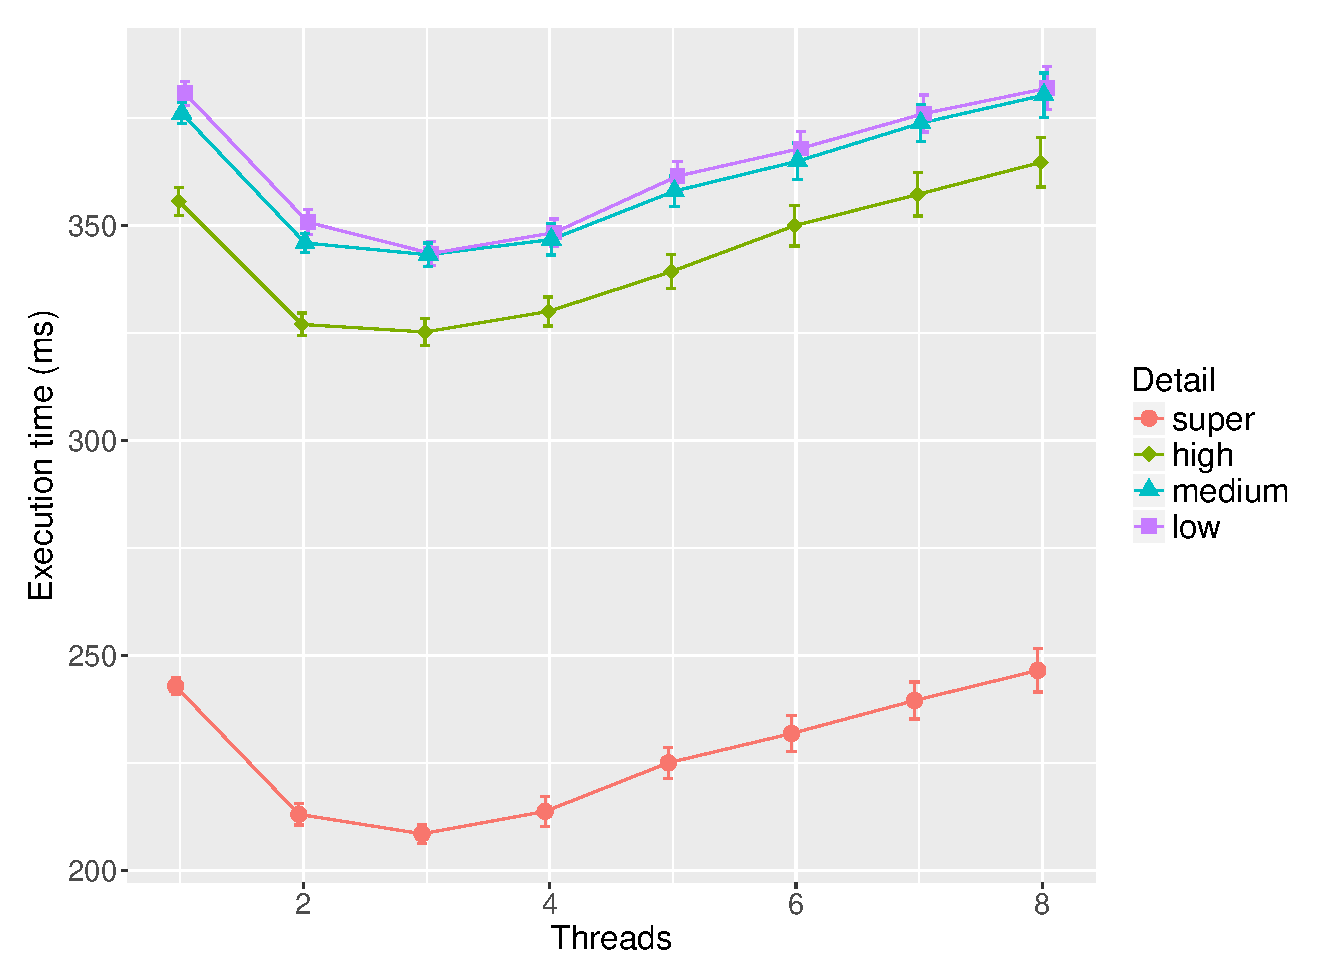
\includegraphics[width=.9\linewidth]{Rdata/parallel_execution_time.eps}
\end{frame}

% texture repair
\begin{frame}
  \begin{figure}
    \subfloat[Original]{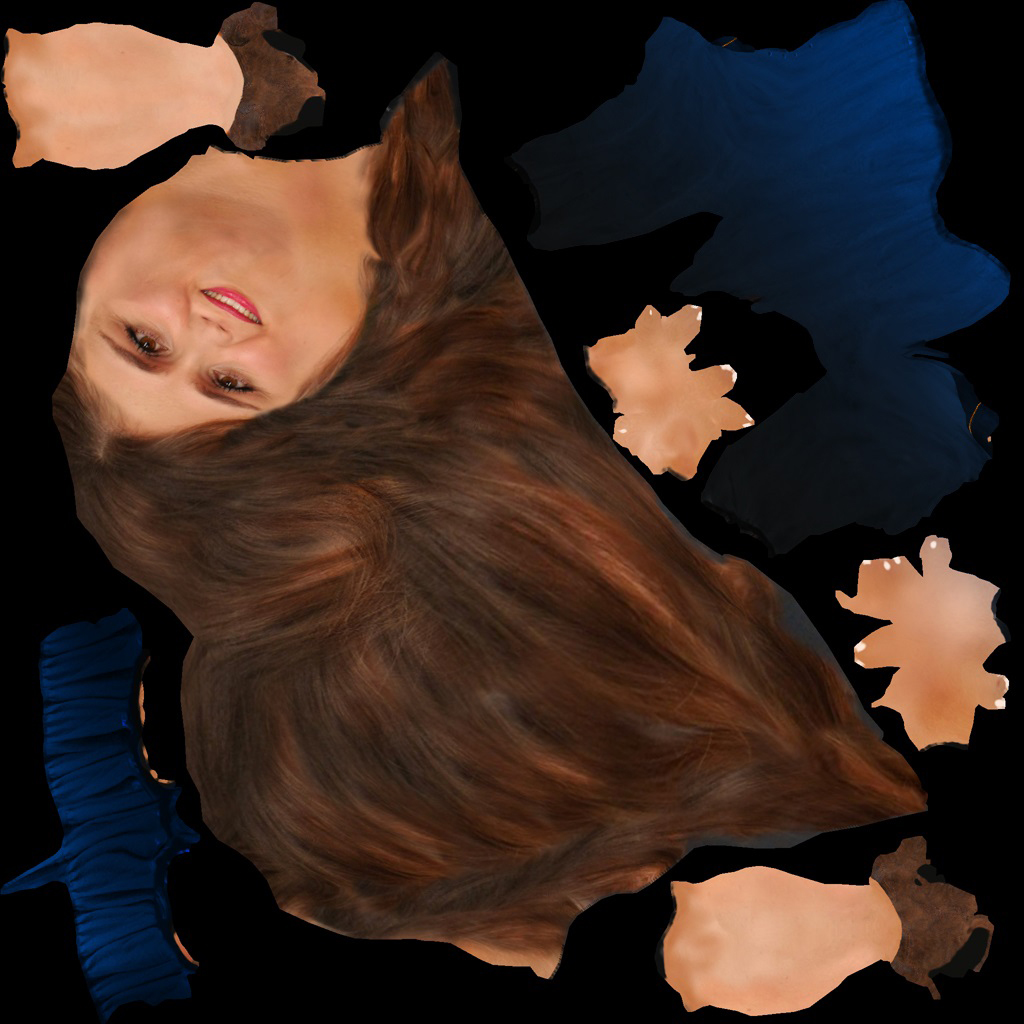
\includegraphics[width=.3\linewidth]{woman_input.jpg}}
    ~
    \subfloat[Bound]{
\includegraphics[width=.3\linewidth]{woman_bound.png}}
    ~
    \subfloat[Improved]{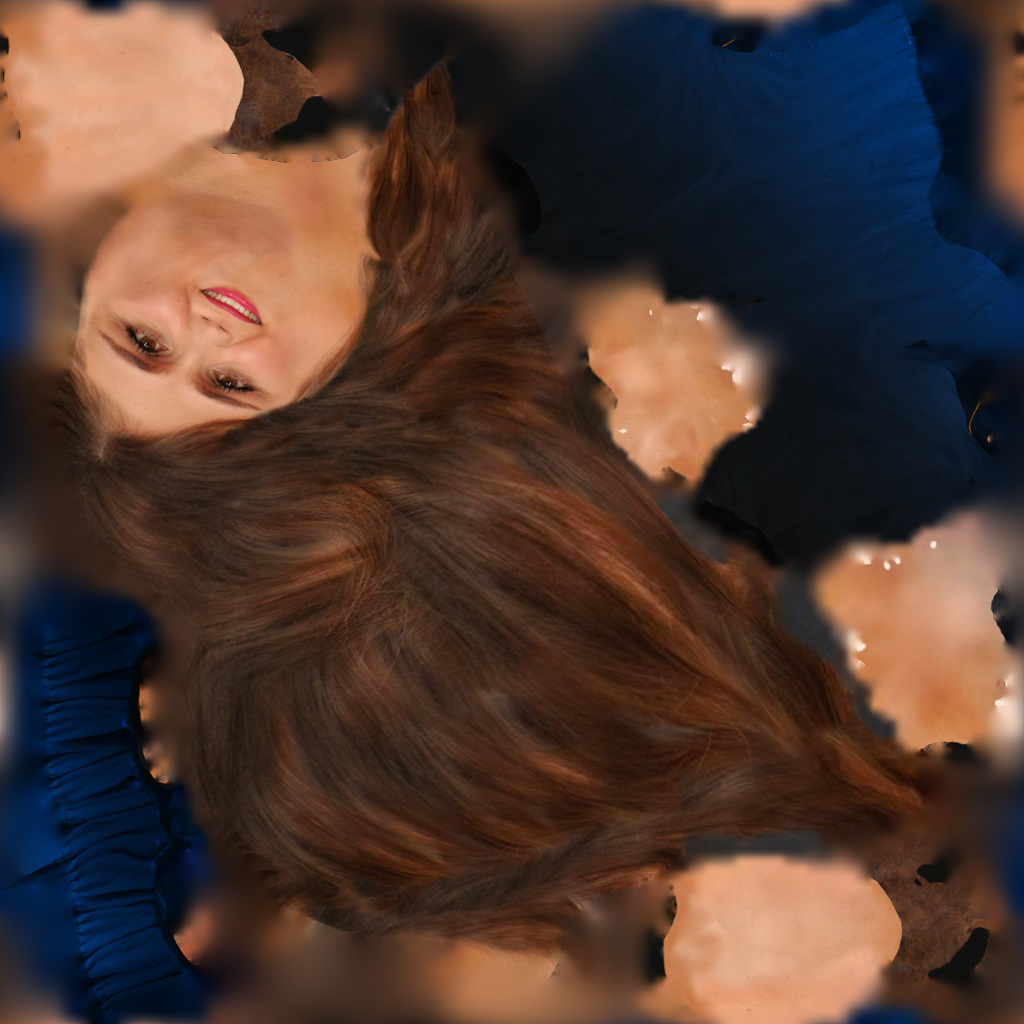
\includegraphics[width=.3\linewidth]{woman_output.png}}
  \end{figure}
\end{frame}

\begin{frame}
  \begin{figure}
    \subfloat{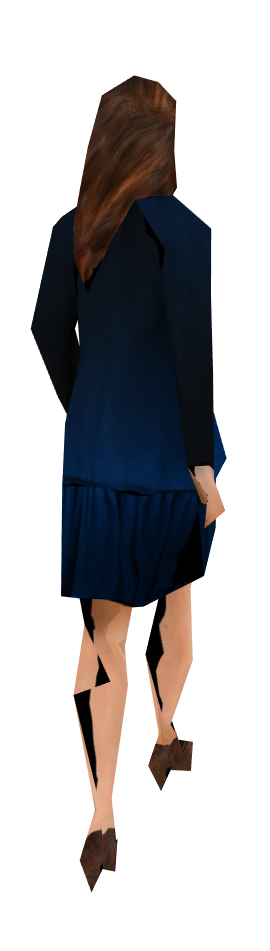
\includegraphics[width=.2\linewidth]{woman_render.png}}
    ~~~~
    \subfloat{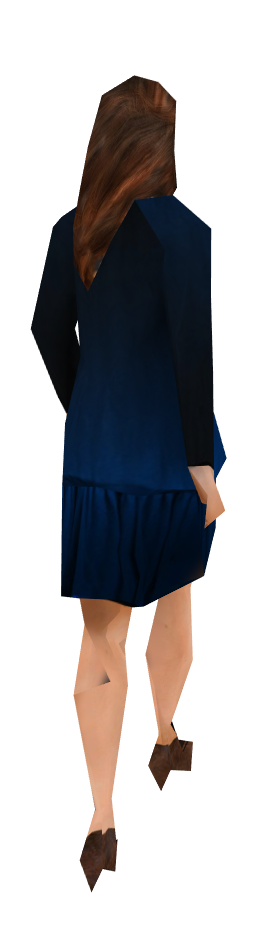
\includegraphics[width=.2\linewidth]{woman_render_improved.png}}
  \end{figure}
\end{frame}

\begin{frame}
  \begin{figure}
    \subfloat[Super]{\includegraphics[width=.2\linewidth]{woman/equal_distance/1.png}}
    ~
    \subfloat[High]{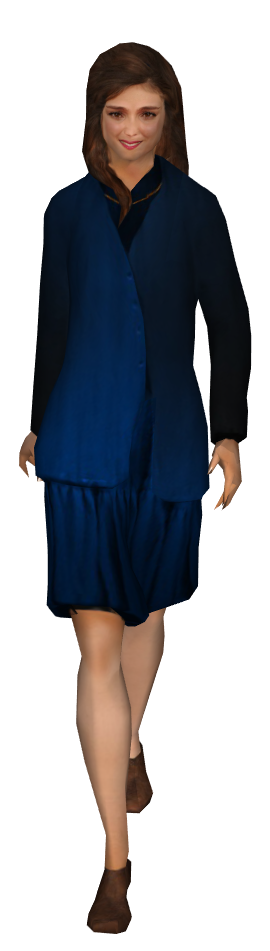
\includegraphics[width=.2\linewidth]{woman/equal_distance/2.png}}
    ~
    \subfloat[Medium]{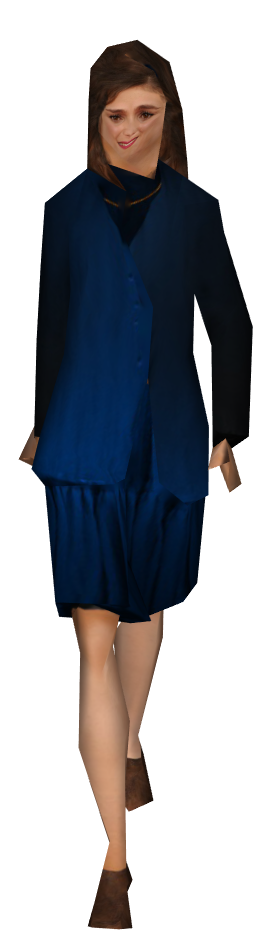
\includegraphics[width=.2\linewidth]{woman/equal_distance/3.png}}
    ~
    \subfloat[Low]{
\includegraphics[width=.2\linewidth]{woman/equal_distance/4.png}}
  \end{figure}
\end{frame}

\begin{frame}
  \begin{figure}
    \subfloat[Super]{\includegraphics[width=.2\linewidth]{woman/cropped/1.png}}
    ~
    \subfloat[High]{
\includegraphics[width=.2\linewidth]{woman/cropped/2.png}}
    ~
    \subfloat[Medium]{
\includegraphics[width=.2\linewidth]{woman/cropped/3.png}}
    ~
    \subfloat[Low]{
\includegraphics[width=.2\linewidth]{woman/cropped/4.png}}
  \end{figure}
\end{frame}

\iffalse

\begin{frame}
  \includegraphics[]{}
\end{frame}

% mesh
\begin{frame}
  \includegraphics[]{}
\end{frame}
\fi



\section*{Summary}

\begin{frame}{Summary}

  \begin{itemize}
  \item
    The \alert{first main message} of your talk in one or two lines.
  \item
    The \alert{second main message} of your talk in one or two lines.
  \item
    Perhaps a \alert{third message}, but not more than that.
  \end{itemize}
  
  % The following outlook is optional.
  \vskip0pt plus.5fill
  \begin{itemize}
  \item
    Outlook
    \begin{itemize}
    \item
      Something you haven't solved.
    \item
      Something else you haven't solved.
    \end{itemize}
  \end{itemize}
\end{frame}


\end{document}


